\documentclass[a4paper]{article}
\usepackage{import}
\usepackage[utf8]{inputenc}
\usepackage[T1]{fontenc}
\usepackage{textcomp}
\usepackage[italian]{babel}
\usepackage{amsmath, amssymb}
\usepackage{booktabs,xltabular}
\usepackage{amsfonts}
\usepackage{subcaption}
\usepackage{amsthm}
\usepackage{cancel}
\usepackage{mdframed}
\usepackage{makecell}
\usepackage{float}
\usepackage{xcolor}
\usepackage{listings}
\usepackage{gensymb}
\usepackage{graphicx}
\usepackage{bodeplot}
\usepackage{physics}
\usepackage{tikz}
\usetikzlibrary{shapes, arrows, automata, petri, decorations.markings, decorations.pathreplacing, positioning, calc, quotes}
\usepackage{circuitikz}
\usepackage[label=corner]{karnaugh-map}
\graphicspath{{./figures/}}

% Set default font to sans-serif
\renewcommand{\familydefault}{\sfdefault} 
\usepackage{eulervm}

\usepackage{forest}

\usepackage{mathtools}
\DeclarePairedDelimiter\ceil{\lceil}{\rceil}
\DeclarePairedDelimiter\floor{\lfloor}{\rfloor}

% \usepackage{ntheorem}

\usepackage{import}
\usepackage{pdfpages}
\usepackage{transparent}
\usepackage{xcolor}

\usepackage{hyperref}
\hypersetup{
    colorlinks=false,
}

% Code blocks
\definecolor{codegreen}{rgb}{0,0.6,0}
\definecolor{codegray}{rgb}{0.5,0.5,0.5}
\definecolor{codepurple}{rgb}{0.58,0,0.82}
\definecolor{backcolour}{rgb}{0.95,0.95,0.95}

\lstdefinestyle{mystyle}{
	backgroundcolor=\color{backcolour},
	commentstyle=\color{codegreen},
	keywordstyle=\color{magenta},
	numberstyle=\tiny\color{codegray},
	stringstyle=\color{codepurple},
	basicstyle=\ttfamily\footnotesize,
	breakatwhitespace=false,
	breaklines=true,
	captionpos=b,
	keepspaces=true,
	numbers=left,
	numbersep=5pt,
	showspaces=false,
	showstringspaces=false,
	showtabs=false,
	tabsize=2
}

\lstset{style=mystyle}

\usepackage{color}
\usepackage{import}
\usepackage{pdfpages}
\usepackage{transparent}
\usepackage{xcolor}

% Example frame
\theoremstyle{definition}
\newmdtheoremenv[%
	linecolor=gray,leftmargin=0,%
	rightmargin=0,
	innertopmargin=8pt,%
	innerbottommargin=8pt,
	ntheorem]{example}{Esempio}[section]

% Important definition frame
\theoremstyle{definition}
\newmdtheoremenv[%
	linecolor=gray,leftmargin=0,%
	rightmargin=0,
	backgroundcolor=gray!40,%
	innertopmargin=8pt,%
	innerbottommargin=8pt,
	ntheorem]{definition}{Definizione}[section]

% Exercise frame
\theoremstyle{definition}
\newmdtheoremenv[%
	linecolor=gray,leftmargin=0,%
	rightmargin=0,
	innertopmargin=8pt,%
	innerbottommargin=8pt,
	ntheorem]{exercise}{Esercizio}[section]

% Theorem frame
\theoremstyle{definition}
\newmdtheoremenv[%
  linecolor=gray,leftmargin=0,%
  rightmargin=0,
  innertopmargin=8pt,%
  innerbottommargin=8pt,
  ntheorem]{theorem}{Teorema}[section]

\theoremstyle{definition}
\newmdtheoremenv[%
  linecolor=white,leftmargin=0,%
  rightmargin=0,
  innertopmargin=8pt,%
  innerbottommargin=8pt,
  ntheorem]{define}{Definizione utile}[section]

% figure support
\usepackage{import}
\usepackage{xifthen}
\pdfminorversion=7
\usepackage{pdfpages}
\usepackage{transparent}
\newcommand{\incfig}[1]{%
	\def\svgwidth{\columnwidth}
	\import{./figures/}{#1.pdf_tex}
}

% FSM tikz
\tikzset{
    place/.style={
        circle,
        thick,
        draw=black,
        minimum size=6mm,
    },
        state/.style={
        circle,
        thick,
        draw=black,
        fill=white,
        minimum size=6mm,
    },
}

\pdfsuppresswarningpagegroup=1

\usepackage{pgfplots}
\pgfplotsset{compat=1.18,width=10cm}

% Save plots as pdf and reuse them without compiling every time
\usetikzlibrary{external}
\tikzexternalize[prefix=figures/tikz/, optimize=false]


\begin{document}

\begin{titlepage}
	\begin{center}
		\vspace*{1cm}

		\Huge
		\textbf{Probabilità e Statistica\\Esercizi}

		\vspace{0.5cm}
		\LARGE
		UniVR - Dipartimento di Informatica

		\vspace{1.5cm}

		\textbf{Fabio Irimie}

		\vfill


		\vspace{0.8cm}


		2° Semestre 2023/2024

	\end{center}
\end{titlepage}


\tableofcontents
\pagebreak

\section{Indirizzamento}
\subsection{Esercizio 1}
Qual'è l'indirizzo di rete se ho il seguente indirizzo IP:
\[
  140.120.84.20/20
\] 

\subsubsection{Risoluzione}
L'indirizzo di rete corrisponde ai primi 20 bit dell'indirizzo IP, quindi bisogna
passare alla notazione binaria:
\[
  140.120.84.20 \to 10001100 \;\; 01111000 \;\; 01010100 \;\; 00010100
\] 
I primi 20 bit sono assegnati al prefisso:
\[
  \underbrace{10001100 \;\; 01111000 \;\; 0101}_{\text{Prefisso}} \;\;
  \underbrace{0100 \;\; 00010100}_{\text{Suffisso}}
\] 
Per ottenere l'indirizzo di rete bisogna azzerare i bit del suffisso:
\[
  \underbrace{10001100 \;\; 01111000 \;\; 0101}_{\text{Prefisso}} \;\;
  \underbrace{0000 \;\; 00000000}_{\text{Suffisso}}
\] 
che in notazione decimale puntata diventa:
\[
  140.120.80.0
\] 
La maschera di questo IP è:
\[
  \underbrace{11111111 \;\; 11111111 \;\; 1111}_{\text{Prefisso}} \;\;
  \underbrace{0000 \;\; 00000000}_{\text{Suffisso}}
\] 
che in notazione decimale puntata diventa:
\[
  255.255.240.0
\] 

\subsection{Esercizio 2}
Si hanno 3 LAN. All'insieme delle 3 LAN è stato assegnato il blocco:
\[
  165.5.1.0/24
\] 
Creare 3 sottoreti per le 3 LAN in modo che abbiano tutte lo stesso numero di host.

\subsubsection{Risoluzione}
Per prima cosa si trasforma l'indirizzo IP in notazione binaria:
\[
  \underbrace{1010 0101 \;\; 0000 0101 \;\; 0000 0001}_{\text{Prefisso}} \;\;
  \underbrace{0000 0000}_{\text{Suffisso}}
\] 
Per poter ottenere 3 sottoreti di dimensione servono 2 bit che vengoo presi dal suffisso
per identificare ciascuna delle 3 reti:
\[
  \underbrace{1010 0101 \;\; 0000 0101 \;\; 0000 0001}_{\text{Prefisso}} \;
  \underbrace{00}_{\text{Sottorete}} \;
  \underbrace{00 0000}_{\text{Suffisso}}
\] 
Le combinazioni possibili sono:
\begin{itemize}
  \item 
    \(
    \underbrace{1010 0101 \;\; 0000 0101 \;\; 0000 0001}_{\text{Prefisso}} \;
    \underbrace{00}_{\text{Sottorete}} \;
    \underbrace{00 0000}_{\text{Suffisso}}
    \) 

  \item 
    \(
    \underbrace{1010 0101 \;\; 0000 0101 \;\; 0000 0001}_{\text{Prefisso}} \;
    \underbrace{01}_{\text{Sottorete}} \;
    \underbrace{00 0000}_{\text{Suffisso}}
    \) 

  \item 
    \(
    \underbrace{1010 0101 \;\; 0000 0101 \;\; 0000 0001}_{\text{Prefisso}} \;
    \underbrace{10}_{\text{Sottorete}} \;
    \underbrace{00 0000}_{\text{Suffisso}}
    \) 

  \item 
    \(
    \underbrace{1010 0101 \;\; 0000 0101 \;\; 0000 0001}_{\text{Prefisso}} \;
    \underbrace{11}_{\text{Sottorete}} \;
    \underbrace{00 0000}_{\text{Suffisso}}
    \) 
\end{itemize}
Ci troviamo con 4 sottoreti con lo stesso numero di indirizzi \( \left( 2^6 = 64 \right) \).
Di queste 4 sottoreti ne utilizziamo 3 e l'ultima rimane libera per utilizzi futuri.

\vspace{1em}
\noindent
Traducendo i blocchi in notazione decimale puntata si ha:
\[
  \begin{aligned}
    165.5.1.0/26 \to \text{LAN 1}\\
    165.5.1.64/26 \to \text{LAN 2}\\
    165.5.1.128/26 \to \text{LAN 3}\\
    165.5.1.192/26 \to \text{Libero}
  \end{aligned}
\] 

\subsection{Esercizio 3}
Usando lo stesso blocco dell'esercizio 2 si modifichi la LAN 1 affinchè abbia il doppio
degli indirizzi rispetto a quelli assegnati alle altre 2 LAN.

\subsubsection{Risoluzione}
Il blocco di partenza in notazione binaria è:
\[
  10100101 \;\; 00000101 \;\; 00000001 \;\; 00000000
\] 
Per ottenere il doppio degli indirizzi rispetto alle altre 2 LAN bisogna prendere un bit
dal suffisso e assegnarlo al prefisso ottenendo così 2 reti /25.
\[
  \begin{aligned}
    \underbrace{1010 0101 \;\; 0000 0101 \;\; 0000 0001}_{\text{Prefisso}} \;
    \underbrace{0}_{\text{Sottorete}} \;
    \underbrace{000 0000}_{\text{Suffisso}}\\
    \underbrace{1010 0101 \;\; 0000 0101 \;\; 0000 0001}_{\text{Prefisso}} \;
    \underbrace{1}_{\text{Sottorete}} \;
    \underbrace{000 0000}_{\text{Suffisso}}
  \end{aligned}
\]
Dalla rete si fa la stessa operazione separando un bit dal suffisso e ottenendo altri 
2 blocchi da /26.
\[
\begin{aligned}
    \underbrace{1010 0101 \;\; 0000 0101 \;\; 0000 0001}_{\text{Prefisso}} \;
    \underbrace{0}_{\text{Lan 1}} \;
    \underbrace{000 0000}_{\text{Suffisso}}\\
    \underbrace{1010 0101 \;\; 0000 0101 \;\; 0000 0001}_{\text{Prefisso}} \;
    \underbrace{10}_{\text{Lan 2}} \;
    \underbrace{00 0000}_{\text{Suffisso}}\\
    \underbrace{1010 0101 \;\; 0000 0101 \;\; 0000 0001}_{\text{Prefisso}} \;
    \underbrace{11}_{\text{Lan 3}} \;
    \underbrace{00 0000}_{\text{Suffisso}}
\end{aligned}
\] 
Traducendo i blocchi in notazione decimale puntata si ha:
\[
  \begin{aligned}
    \text{Lan 1: } & 165.5.1.0/25\\
    \text{Lan 2: } & 165.5.1.128/26\\
    \text{Lan 3: } & 165.5.1.192/26
  \end{aligned}
\] 

\subsection{Esercizio 4}
Si consideri la seguente rete suddivisa in 5 sottoreti:
\begin{figure}[H]
  \centering
  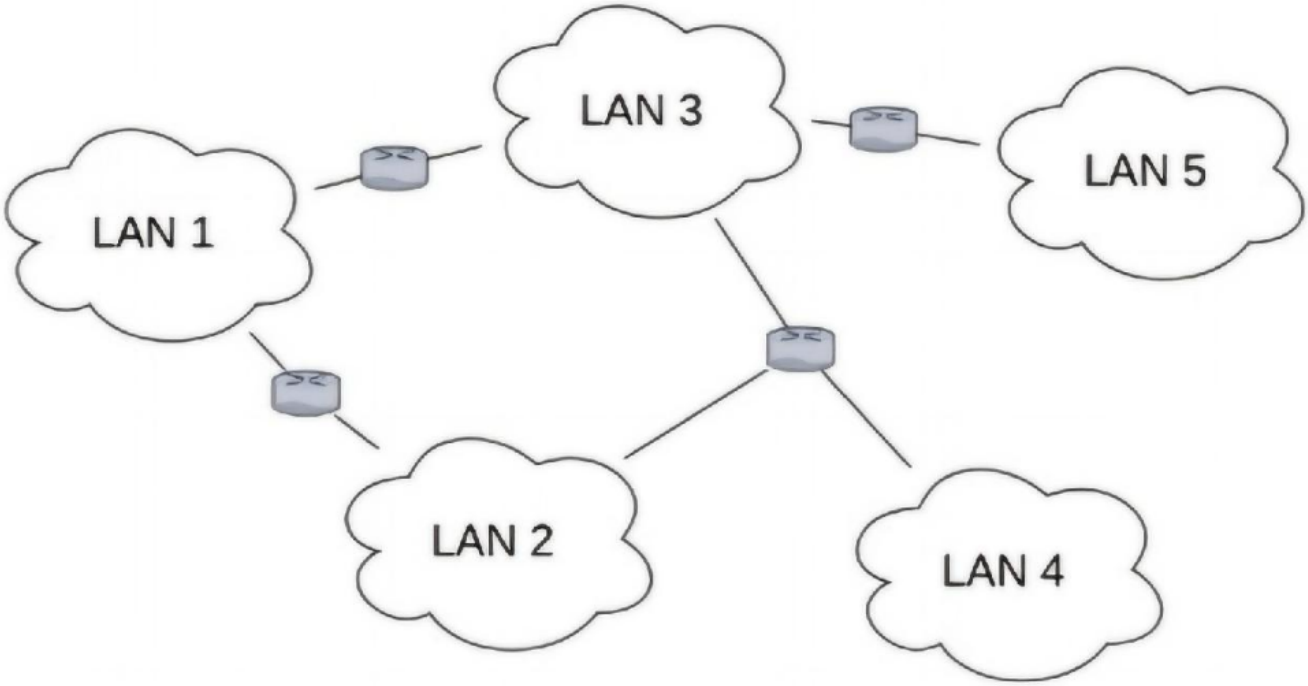
\includegraphics[width=0.75\textwidth]{../figures/esercitazione-es1}
\end{figure}

\noindent
Ci sono due indirizzi già assegnati alla rete:
\begin{itemize}
  \item 101.75.79.255
  \item 101.75.80.0
\end{itemize}

\begin{enumerate}
  \item Qual'è il blocco \textbf{CIDR} più piccolo (con il minor numero di indirizzi) che
    contiene tali indirizzi?
  \item Dato il blocco \textbf{CIDR} della domanda precedente, si creino 5 sottoreti con
    i seguenti vincoli:
\begin{itemize}
  \item \textbf{LAN 1}: deve essere una sottorete /21

  \item \textbf{LAN 2}: deve ospitare fino a 1000 host

  \item \textbf{LAN 3}: deve essere una sottorete /23
  \item \textbf{LAN 4}: deve ospitare fino a 400 host

  \item \textbf{LAN 5}: deve ospitare metà host rispetto al blocco iniziale
\end{itemize}
\end{enumerate}

\subsubsection{Risoluzione}
\begin{enumerate}
  \item 
    Converto entrambi gli indirizzi in notazione binaria:
    \[
      \begin{aligned}
        101.75.79.255 & \to 01100101 \;\; 01001011 \;\; 01001111 \;\; 11111111 \\
        101.75.80.0   & \to 01100101 \;\; 01001011 \;\; 01010000 \;\; 00000000
      \end{aligned}
    \] 
    Siccome i due IP sono uguali fino al 19° bit a partire da sinistra, si può dire che
    il blocco CIDR più piccolo che contiene entrambi gli indirizzi sia quello della rete:
    \[
      \underbrace{01100101 \;\; 01001011 \;\; 010}_{\text{Prefisso}}
      \;\; \underbrace{00000 \;\; 00000000}_{\text{Suffisso}}
    \]
    che in notazione intera puntata è il seguente:
    \[
      101.75.64.0/19
    \] 

  \item 
    \begin{itemize}
      \item \textbf{LAN 1}:

    \vspace{1em}
    \noindent
    Per avere una sottorete /21 basta spostare i bit del prefisso:
    \[
      \underbrace{01100101 \;\; 01001011 \;\; 010}_{\text{Prefisso}}
      \;\; \underbrace{00000 \;\; 00000000}_{\text{Suffisso}}\\
    \]
    \[
      \Downarrow
    \]
    \[
      \underbrace{01100101 \;\; 01001011 \;\; 01000}_{\text{Prefisso}}
      \;\; \underbrace{000 \;\; 00000000}_{\text{Suffisso}}\\
    \] 
    che in notazione intera puntata risulta:
    \[
      101.75.64.0/21
    \] 

  \item \textbf{LAN 2}:

    \vspace{1em}
    \noindent
    1000 host sono circa \( 2^{10} \), di conseguenza per avere un blocco che possa
    ospitare fino a 1000 host esso deve avere almeno 10 bit di suffisso:
    \[
      \underbrace{01100101 \;\; 01001011 \;\; 010000}_{\text{Prefisso}}
      \;\; \underbrace{00 \;\; 00000000}_{\text{Suffisso}}\\
    \] 
    che in notazione intera puntata risulta:
    \[
      101.75.64.0/22
    \] 

  \item \textbf{LAN 3}:

    \vspace{1em}
    \noindent
    Per avere una sottorete /23 basta spostare i bit del prefisso:
    \[
      \underbrace{01100101 \;\; 01001011 \;\; 010}_{\text{Prefisso}}
      \;\; \underbrace{00000 \;\; 00000000}_{\text{Suffisso}}\\
    \]
    \[
      \Downarrow
    \]
    \[
      \underbrace{01100101 \;\; 01001011 \;\; 0100000}_{\text{Prefisso}}
      \;\; \underbrace{0 \;\; 00000000}_{\text{Suffisso}}\\
    \] 
    che in notazione intera puntata risulta:
    \[
      101.75.64.0/23
    \] 


  \item \textbf{LAN 4}:

    \vspace{1em}
    \noindent
    400 host sono circa \( 2^{9} \), di conseguenza per avere un blocco che possa
    ospitare fino a 400 host esso deve avere almeno 9 bit di suffisso:
    \[
      \underbrace{01100101 \;\; 01001011 \;\; 0100000}_{\text{Prefisso}}
      \;\; \underbrace{0 \;\; 00000000}_{\text{Suffisso}}\\
    \] 
    che in notazione intera puntata risulta:
    \[
      101.75.64.0/23
    \] 

  \item \textbf{LAN 5}:

    \vspace{1em}
    \noindent
    Il blocco iniziale riesce ad ospitare \( 2^{13} \) host, quindi per creare una rete
    che ne ospiti la metà bisogna avere \( \frac{2^{13}}{2} = 2^{13-1} = 2^{12} \) 12
    bit di suffisso:
    \[
      \underbrace{01100101 \;\; 01001011 \;\; 0100}_{\text{Prefisso}}
      \;\; \underbrace{0000 \;\; 00000000}_{\text{Suffisso}}\\
    \] 
    che in notazione intera puntata risulta:
    \[
      101.75.64.0/20
    \] 
\end{itemize}
\end{enumerate}

\subsection{Esercizio 5}
Si hanno 3 LAN con i seguenti numeri di host:
\begin{enumerate}
  \item LAN 1: 300 host
  \item LAN 2: 40 host
  \item LAN 3: 90 host
\end{enumerate}
L'indirizzo di broadcast della LAN 3 è:
\[
148.12.79.255
\] 
\begin{enumerate}
  \item Trovare il blocco CIDR totale da assegnare all'intera rete
  \item Partendo da tale blocco suddividerlo in sottoreti da assegnare alle 3 LAN
\end{enumerate}

\subsubsection{Risoluzione}
\begin{enumerate}
  \item 
    Per trovare il blocco CIDR totale bisogna trovare il blocco che riesce a contenere
    il numero di host totale (in base 2) delle 3 LAN:
    \[
      512 + 64 + 128 = 704
    \] 
    Il blocco CIDR che riesce a contenere 704 host è:
    \[
      2^{10} = 1024
    \] 
    Di conseguenza il blocco CIDR totale dovrà avere 10 bit di suffisso e l'indirizzo di
    rete si ottiene convertendo l'indirizzo di broadcast in notazione binaria e azzerando
    i bit del suffisso:
    \[
      \underbrace{1001 0100 \;\; 0000 1100 \;\; 0100 11}_{\text{Prefisso}}
      \;\; \underbrace{00 \;\; 00000000}_{\text{Suffisso}}
    \] 
    che in decimale risulta:
    \[
      148.12.76.0/22
    \] 

  \item 
    Per suddividere il blocco CIDR in 3 sottoreti bisogna trovare il numero di bit di
    suffisso necessari per contenere il numero di host di ciascuna LAN:
    \begin{itemize}
      \item LAN 1: 300 host, \( 2^9 = 512 \) quindi 9 bit di suffisso
      \item LAN 2: 40 host, \( 2^6 = 64 \) quindi 6 bit di suffisso
      \item LAN 3: 90 host, \( 2^7 = 128 \) quindi 7 bit di suffisso
    \end{itemize}
    Quindi il blocco CIDR totale:
    \[
      \underbrace{1001 0100 \;\; 0000 1100 \;\; 0100 11}_{\text{Prefisso}}
      \;\; \underbrace{00 \;\; 00000000}_{\text{Suffisso}}
    \] 
    verrà suddiviso in:
    \[
      \begin{aligned}
        \text{LAN 1: } &
        \underbrace{1001 0100 \;\; 0000 1100 \;\; 0100 11}_{\text{Prefisso}}
        \;\; \underbrace{0}_{\text{Lan 1}}
        \;\; \underbrace{0\;\;00000000}_{\text{Suffisso}}\\
        \text{LAN 2: } &
        \underbrace{1001 0100 \;\; 0000 1100 \;\; 0100 11}_{\text{Prefisso}}
        \;\; \underbrace{11\;\;01}_{\text{Lan 2}}
        \;\; \underbrace{000000}_{\text{Suffisso}}\\
        \text{LAN 3: } &
        \underbrace{1001 0100 \;\; 0000 1100 \;\; 0100 11}_{\text{Prefisso}}
        \;\; \underbrace{11\;\;1}_{\text{Lan 3}}
        \;\; \underbrace{0000000}_{\text{Suffisso}}\\
      \end{aligned}
    \]
    che in notazione puntata risultano:
    \[
    \begin{aligned}
      \text{LAN 1: } & 148.12.76.0/23\\
      \text{LAN 2: } & 148.12.79.64/26\\
      \text{LAN 3: } & 148.12.79.128/25
    \end{aligned}
    \] 
\end{enumerate}

\section{TCP}
L'obiettivo di questi esercizi è quello di vedere come si comporta l'algoritmo in situazioni 
particolari.
\subsection{Esercizio 1}
Un'applicazione \( A \) deve trasferire verso un'applicazione \( B \) \( 96000 byte \).
Si suppone che la connessione sia già stata instaurata. I dati sono i seguenti:
\begin{itemize}
  \item \texttt{mss} = 1000 byte
  \item \texttt{rcvwnd} = 32000 byte, costante per l'intero trasferimento dei dati
  \item \texttt{ssthresh} = \( \frac{\texttt{rcvwnd}_{\text{iniziale}}}{2} \) 
  \item \texttt{rtt} = costante, pari a \( 0.5 \) secondi
  \item \texttt{rto} = \( 2 \cdot \texttt{rtt} \), raddoppia in caso di perdite sequenziali
  \item Down di rete (rete fuori uso, in cui tutti i segmenti vengono persi) = 
    \[
    \begin{aligned}
      t_1 = 3 &\to t_2 = 3,5\\
      t_3 = 7 &\to t_4 = 7,5
    \end{aligned}
    \] 
\end{itemize}
Lo scopo è quello di valutare l'evoluzione temporale della \texttt{cwnd} fino a fine
trasmissione.

\subsubsection{Risoluzione}
Il numero di segmenti da trasmettere sono:
\[
  \frac{\text{byte da trasmettere}}{\text{\texttt{mss}}} = \frac{96000 byte}{1000 byte}
  = 96 \text{ segmenti}
\] 
La \texttt{rcvwnd} iniziale vale:
\[
  \text{\texttt{rcvwnd}}_{\text{iniziale}} = \frac{32000 byte}{1000 byte} = 32 \text{ segmenti}
\] 
La \texttt{ssthresh} vale:
\[
  \text{\texttt{ssthresh}}_{\text{iniziale}} = \frac{32}{2} = 16 \text{ segmenti}
\]
La \texttt{cwnd} iniziale vale 1:
\[
  \text{\texttt{cwnd}}_{\text{iniziale}} = 1
\] 
\label{12-11-D4}



\end{document}
